\chapter{Desarrollo e Implementación}

\section{Hardware}

El hardware se diseña por medio del software Proteus ...

\section{Firmware}

El firmware se desarrolla sobre el framework o SDK oficial de Espressif Systems, ESP-IDF el cual posee una documentación \cite{ES}, la cuál es muy útil a la hora de utilizar las diferentes APIs que este posee.\\

Sobre el firmware se desarrollan los siguientes temas:

\paragraph{GPIO:}

el ESP-WROOM-32 posee diferentes GPIO, los cuales se usan para leer o escribir señales digitales, en cuanto a los sensores se pueden enviar señales para iniciar su lectura o simplemente tener el pin en modo entrada y leerlo cada cierto intervalo de tiempo para generar la lectura, o en modo salida para el control de los diferentes dispositivos que se han desarrollado en el hardware.

\paragraph{ADC:}

se usan para leer los datos de algunos sensores que dan una salida analogica, por este motivo se hace la conversion de la señal analogica a un valor digital dentro de la tarjeta, para luego identificar el valor de la lectura del sensor. 

\paragraph{Consola:}

para realizar diferentes pruebas directamente desde la tarjeta, se usa la opción de la consola que se comunica por medio del puerto serie, para esto se crean las funciones y los comandos que estaran disponibles. Algunos comandos disponibles son \textit{http}, para realizar las peticiones http manualmente y observar su respuesta, pin para realizar la prueba de un pin digital como entrada o salida, \textit{help} para observar la lista de comandos, entre otros.

\paragraph{HTTP Request:}

las peticiones HTTP son indispensables en estas aplicaciones del campo IOT, por este motivo en el desarrollo del firmware se usan las librerias pertinentes para realizar peticiones y además leer las respuestas de estas desde el servidor, ya que este es el medio de comunicación tarjeta-servidor.

\paragraph{Tareas:}

se desarrollan diferentes tareas para la lectura y la escritura en los diferentes puerto de la tarjeta, la tareas son propias de los sistema operativos.

\paragraph{Timers:}

son utilizados principalmente para el control de cargas AC ...

\paragraph{I2C:}

el protocolo I2C se activa por medio de la instalación del driver en algún par de pines GPIO disponibles en la tarjeta, en esta ocasión se usan los pines 20 y 21 para realizar allí la conexión física del bus de datos de este protocolo, además de esto se crea una tarea la cuál se encarga de solicitar y leer los datos de los diferentes sensores conectados a este.

\paragraph{PWM:}

para controlar las cargas DC se usa una salida PWM, ya que al variar el ancho de pulso este

\paragraph{Interrupciones:}

las interrupciones se usan para no gastar recursos en un monitoreo constante de las entradas, solo cuando exista un cambio de nivel en la entrada el dispositivo desencadena una serie de instrucciones relacionas al tipo de interrupción y a diferentes funciones creadas para esta, la interrupción se usa por medio de los diferentes pines propuestos para esto en el hardware.

\section{Software}

Para el software se utiliza una plataforma como servicio (PaaS) el cuál es el servicio que ofrece la plataforma Heroku, en este caso se usa una cuenta gratuita para realizar las pruebas de la aplicación, allí en el servidor de la plataforma se aloja la aplicación desarrollada en HTML5 y PHP.\\

Por este motivo se usa el framework Laravel, el cual como se menciona anteriormente combina HTML5, PHP y un ORM, para realizar el manejo de toda la parte del servidor se usa PHP, este framework proporciona un mapeo de consultas para las bases de datos, así que las consultas se hacen como codigo de PHP y este se encarga de realizar los comando de SQL necesarios, lo que facilita que la aplicación use diferentes gestores de bases de datos como MySQL, SQLite, entre otras.\\

Para el software se toman en cuenta dos tipos de vista, una vista pública y una privada, como se observa en la figura \ref{fig:index}. En la vista pública se encuentran los datos de contacto, solicitudes de registro o productos y la cantidad de usuarios. En la vista privada se encuentra la interacción de los usuarios y dueños de las casas, para controlar y ver sus datos.\\

\begin{figure}
	\centering
	\caption{Página de Inicio}
	\label{fig:index}
	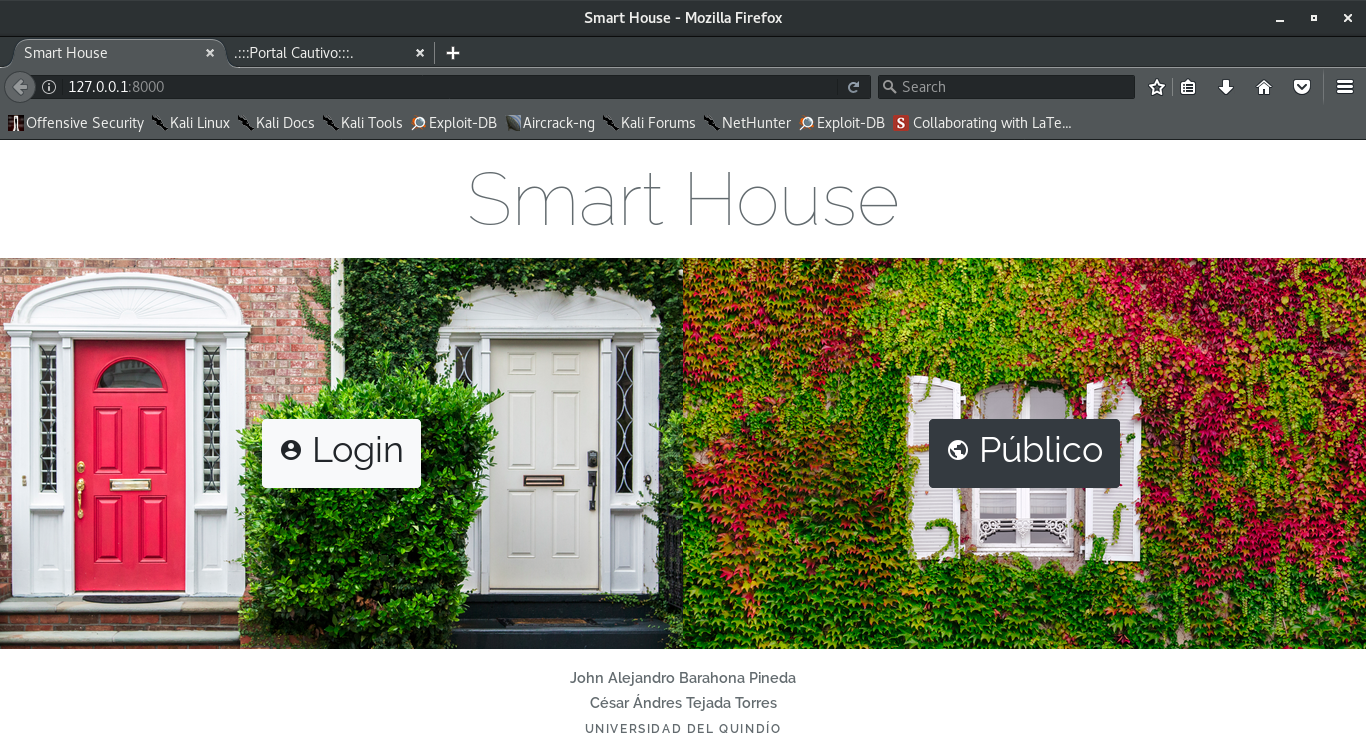
\includegraphics[width=0.9\linewidth]{Imagenes/Index}
\end{figure}


Esta parte se garantiza por medio del framework, creando diferentes roles para cada usuario que se esta registrando y realizando la comprobación por parte del Middleware que provee este.\\

Para el manejo de los diferentes sensores y usuarios todo se registra en la base de datos que facilita la plataforma Heroku.\\

\subsection{Parte Pública}

En esta vista simplemente hay opciones para el contacto y solicitudes, como se menciona anteriormente, es una vista sencilla dada la poca información que contiene, como se observa en la figura \ref{fig:publicview}.

\begin{figure}
	\centering
	\caption{Vista Pública}
	\label{fig:publicview}
	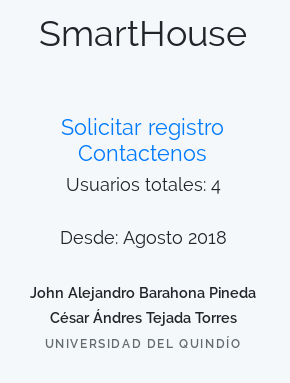
\includegraphics[width=0.9\linewidth]{Imagenes/Public_view}
\end{figure}



\subsection{Parte Privada}

En esta sección es donde se encuentra el Panel de Control para un usuario administrador que son los dueños de la aplicación, la vista se puede observar en la figura \ref{fig:adminview}, usuarios dueños de las diferentes casas que poseen el dispositivo y otro usuario dueño de la habitación donde se encuentra el dispositivo, este ultimo usuario está sujeto a un usuario dueño de la casa, ya que el usuario de la casa puede observar todas las habitaciones mientras que el usuario de habitación solamente le compete su habitación.\\

\begin{figure}
	\centering
	\caption{Vista del Usuario Administrador}
	\label{fig:adminview}
	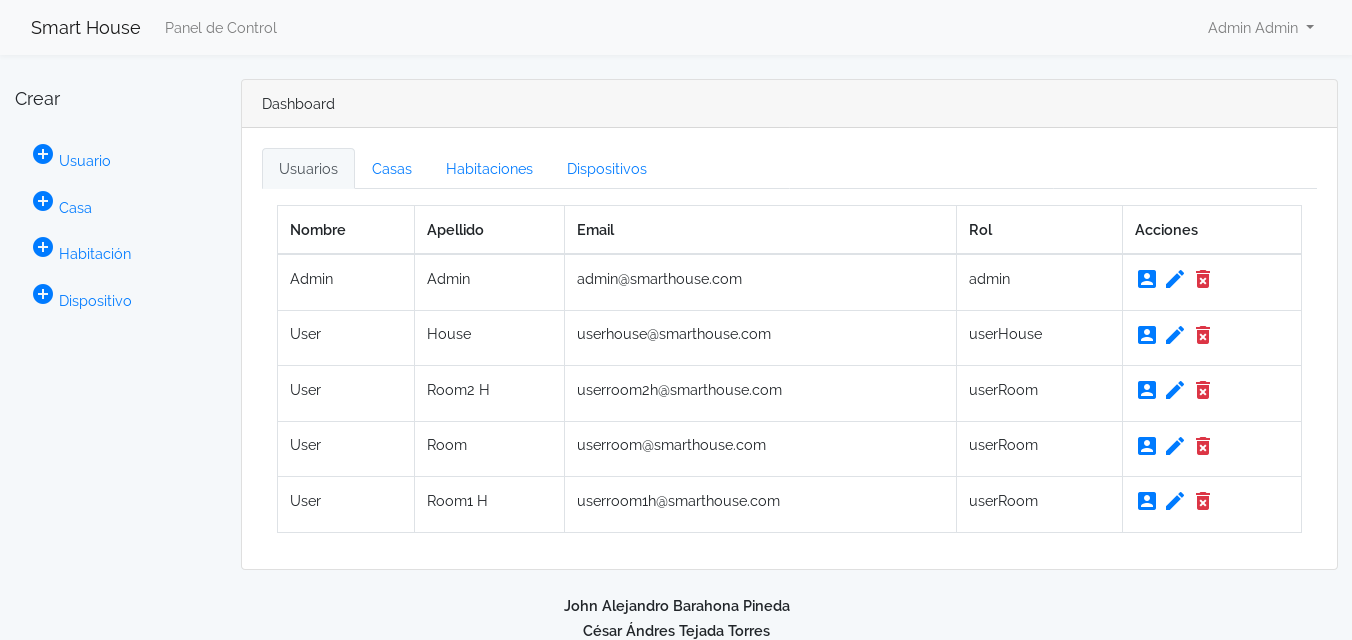
\includegraphics[width=0.9\linewidth]{Imagenes/Admin_view}
\end{figure}

Además de esto en la parte privada se encuentra la pagina encargada de la actualización Servidor-Tarjeta, la cual recibe una petición tipo GET y por medio de la URL añade un texto tipo JSON en el cual se encuentra toda la información de los sensores, y el servidor responde con un texto también tipo JSON con la información pertinente de los actuadores, como se observa la figura \ref{fig:updateview}, esto se identifica mediante un token que esta presente y es unico en los datos de cada habitación.\\

\begin{figure}
	\centering
	\caption{Página de intercambio de datos}
	\label{fig:updateview}
	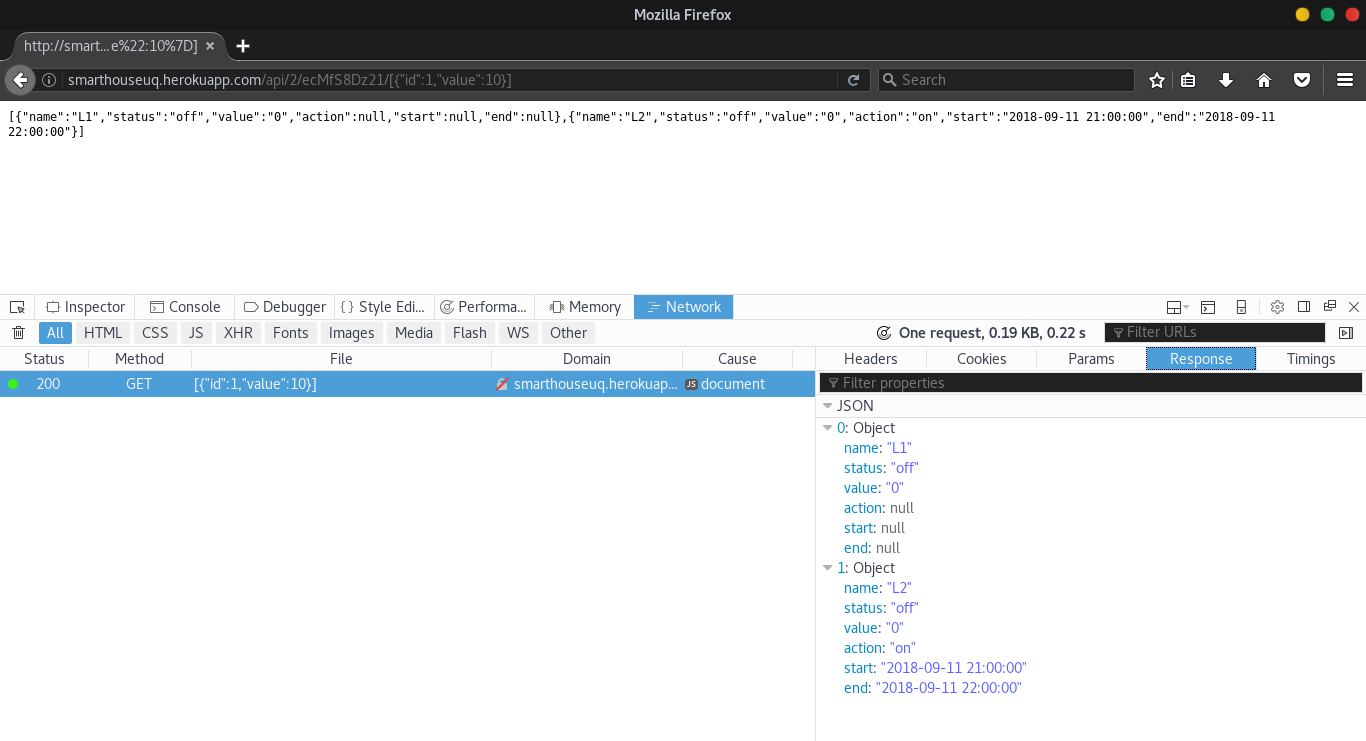
\includegraphics[width=0.9\linewidth]{Imagenes/Update_view}
\end{figure}


\subsection{Base de Datos}

Por medio del framework se crea en la base de datos las siguientes tablas, para guardar la información pertinente, se crea una tabla de usuarios, una tabla de casas, de habitaciones y de dispositivos con las siguientes relaciones como se observa en la figura \ref{fig:db}.\\

\begin{figure}
	\centering
	\caption{Base de datos SmartHouse}
	\label{fig:db}
	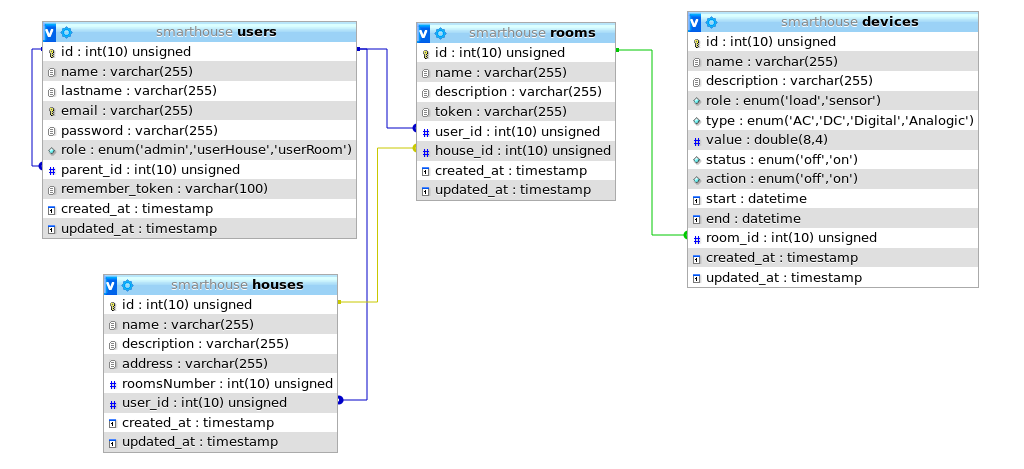
\includegraphics[width=0.7\linewidth]{Imagenes/DB}
\end{figure}
